% !TEX encoding = UTF-8 Unicode
% -*- program: pdflatex -*-
\documentclass[fleqn,10pt,lineno]{wlpeerj}
\usepackage[hidelinks]{hyperref}
\usepackage[T1]{fontenc}
\usepackage{tgtermes}
\usepackage{etoolbox}
\usepackage{graphicx}
\usepackage{subfloat}
\usepackage{comment}
\usepackage{soul}
\hypersetup{
   pdftitle={CVX},
   pdfauthor={Alexa Tyszka, Karolis Ramanauskas, Boris Igi{\'c}}
   }
%\usepackage[all]{hypcap} % NOTE BELOW:
%B: I don't know where this comes from (or who put it here, me, K, A?), but K says it breaks \includegraphics
% If it is used for something important, let me know.
\usepackage{doi} % remove url!
\graphicspath{{figures/}}
\renewcommand{\bibsection}{\section*{References}}
\providecommand{\e}[1]{\ensuremath{\times 10^{#1}}}
\newcommand{\ca}{\textit{ca}.}

%--------------------------------------------------
% How to Handle Supplemental Materials
%--------------------------------------------------

% PeerJ instructions:
%
% Supplemental materials. Online publishing allows inclusion of information that may not fit into a printed paper with page limits or may be deemed redundant (tables of data included in a figure) or otherwise inappropriate for the print version (extensive photographic evidence, metadata, other potentially useful information not essential to the paper). These files are not included in the page/word counts of the manuscript and will be presented online as submitted by the authors (not copy edited). Authors should upload this information as a separate file entitled ?Supplement? in PeerTrack. Text references to this material in the manuscript will be inserted as hotlinks to the online information. Supplemental figure and table numbers should be preceded by the letter S to indicate supplemental (Supplemental Table S1, Supplemental Fig. S4).
%
% Here's what we'll do:
% (1) we'll have another tex file called cvx-cactaceae-suppinfo.tex and we'll insert it for use in this file as follows:
% \externaldocument{cvx-cactaceae-suppinfo.tex}
%
% (2) each figure table will be inserted as usual with \begin{figure} ... \end{figure}
% (3) In the text, you just reference these with their label, as you would any other figure! That's it!

%--------------------------------------------------
% TITLE PAGE
%--------------------------------------------------
\title{Genome evolution, taxonomy, and transmission of potexviruses in cacti (\textit{Alphaflexiviridae})}

\author[1,$\dagger$]{Alexa Tyszka}
\author[1]{Karolis Ramanauskas}
\author[1]{Boris Igi\'c}
\affil[1]{Department of Biological Sciences, University of Illinois at Chicago, 840 West Taylor St.\ MC067, Chicago, IL 60607, United States of America}
 \affil[$\dagger$]{Author for correspondence.}


%\begin{linenumbers}
%\modulolinenumbers[1]
%\setstretch{1.0}

%--------------------------------------------------
% ABSTRACT 
%--------------------------------------------------

\begin{abstract}

\textit{Potexvirus} is a group of positive-sense single-stranded RNA viruses known to infect many flowering plants, including cacti (Cactaceae).
%The viral taxonomic naming schemes in this group are based on the name of the host plant at the time the virus is discovered, thereby resulting in a naming system that does not update with taxonomy. 
The current viral taxonomic naming schemes in this group often employ informal or outdated host plant names (synonyms), which complicate systematic study.
One such group, often named with a suffix "Virus X," presents a further complication---nearly all of its published sequences are from infections of cultivated plants, in which infections may dramatically affect yield.
Because their host-specificity is broad, the source of infections, the natural distribution of this group, and the significance of infections in wild species of cacti all remain unclear.
The lack of clarity is partly related to low sampling across the Potexviruses that infect cacti. 
And yet, the availability of sampled plant transcriptomes, all of which are practically metatranscriptomes, has recently exploded, along with the decreasing expense and difficulty of conducting RNAseq experiments.
Here, we harness these new tools and perform phylogenetic analyses aimed at clarifying taxonomic diversity, quantifying patterns of tissue expression, diversity, and examining selective pressures across viral genomes. 
The results suggest a novel mode of transmission by sex (pollination) for this viral group, based on significant expression in pollen.
We examine and discuss the implications of our key results for the taxonomy of \textit{Potexviruses} that infect Cactaceae, noting their vastly understudied ecological significance.

\end{abstract}

%--------------------------------------------------
\begin{document}
%--------------------------------------------------
%
\flushbottom
\maketitle
\thispagestyle{empty}
%\setlength{\emergencystretch}{7.5pt}
%\setstretch{1.0}
%\setlength{\parindent}{0.25in}


%--------------------------------------------------
\section*{To-do and relevant fixes to be completed before submission}
%--------------------------------------------------
\begin{enumerate}
\item Figure captions need to be expanded and proofread.
\item Some methods and results are patchy and need to be written, and they are \hl{highlighted} as a reminder. 
\item The capitalization and italicization of \textit{Potexvirus} is not as consistent as it could be -- I apologize for this nuisance. When referring to the \textit{Potexvirus} genus or using \textit{Potexvirus} as an adjective, it should be capitalized and italicized. As a noun, such as "potexviruses", it is okay uncapitalized and unitalicized.
\end{enumerate}


%--------------------------------------------------
\section*{Introduction}
%--------------------------------------------------

Molisch's (1885) \nocite{molisch1885} discovery of ``protein bodies'' on several species of cacti was one of the first documented descriptions of viruses.
For nearly a century, subsequent comparative study of viruses remained limited to direct observational data of gross morphology, augmented with clever experimental approaches, such as filtration and inoculation \citep{mettenleiter2017}.
A transformative advancement in virology---and all of biology---has been the advent of massively parallel DNA and RNA sequencing. 
The rapidly improving sequencing tools enable rapid identification of organisms from seemingly any sampled surface of the Earth.
One common thread is that virtually every macro-organism genome study uncovers a micro-organismal metagenome, composed of both targeted host sequences and those from myriad co-existing organisms. 
Metagenomic studies have yielded an enormous number of genomes and have vastly expanded the global viriome \citep{gregory_marine_2019,lefeuvre2019,shi_redefining_2016}. 
%B: this is an unusually large in-line citation set. I would pick one or two transformative studies, not the whole gamut.
The unprecedented amount of data resulting from metagenomic studies has also caused significant policy changes and revisions by the International Committee on Taxonomy of Viruses (ICTV) policy \citep{ictv2020,simmonds2017virus}, but nearly all viruses remain named by their original description of host, location, and/or symptoms.

The historic naming conventions are ill-suited for host plants whose own taxonomic placement is uncertain, which has been particularly true for rapidly diversified groups such as Cactaceae (cacti).
Molisch's ``protein bodies'' are now widely understood to be comprised of plant-infecting potexviruses (\textit{Tymovirales}, family \textit{Alphaflexiviridae}).
Their positive-sense, single-stranded RNA genomes consist of 5.9-7.0 kb of positive-sense single-stranded RNA \citep{martelli_family_2007}.
Generally presenting as elongated, rod-shaped filamentous viruses, they express five primary open reading frames (ORFs): Replicase (Rep), Triple gene block (TGB), Coat protein (CP), coded in the 5' direction as well as two smaller overlapping ORFs coded in the 3' direction: ORF6 and ORF7 \citep{martelli_family_2007}. 
%if one of these citations mentions the structure, it is sufficient.
%at: deleted all but the most relevant citation
%They are closely related to other \textit{Potexviruses} such as \textit{Alternantha Mosaic Virus} and \textit{Papaya Mosaic Virus} \citep{martelli_family_2007,park_detection_2018,liou_complete_2004}.
Members of this group produce variably symptomatic infections in cacti, and many infected plants show no external signs of viral infection \citep{bos_symptoms_1977, liou_complete_2004}. 
Neither the significance of their infections in nature, nor relative modes of transmission are clear. 
Reports of symptomatic plants range from 0\%-5.5\% in wild species in the southwestern United States \citep{attathom_occurrence_1978} to 44\% in agricultural fields on Hainan Island, China \citep{peng_molecular_2016}.
The most commonly recognized symptoms of the disease are mosaic, mottling, stunted growth, and distortion \citep{attathom_occurrence_1978, maliarenko_cactus_2013, peng_molecular_2016}.
Infection through grafting and mechanical contact, particularly following stem injury and human-mediated or hemipteran insect-mediated sap inoculation, is well-documented \citep{liou_complete_2004,maliarenko_cactus_2013,park_detection_2018}.
Grafting is a primary means of propagation among crop cacti \citep{park_detection_2018}, and \textit{Selenicereus} is a commonly chosen graft stock.
However, there are reports of other members within the family \textit{Alphaflexiviridae} transmitting via insect and seed vectors \citep{martelli_family_2007}, and pre-DNA studies tentatively suggest that in the wild, pollen may transmit \textit{CVX} \citep{attathom_occurrence_1978}.

%This paragraph needs a topic sentence: "viral taxonomy is complicated by many aspects of biology and taxonomic practices" or something.
\textit{Schlumbergera truncata} (Haworth) Moran has undergone a number of name changes, including \textit{Epiphyllum truncatum} Haworth in 1819, \textit{Cactus truncatus} (Haworth) Link in 1822, and \textit{Zygocactus truncatus} (Haworth) K. Schumann in 1890, dramatically confusing subsequent viral taxonomy.
%This naming scheme may cause confusion as it results in many distinct viruses having the same name.
Thus, currently accepted names in the \textit{Potexvirus} group include \textit{Cactus Virus X} (CVX), \textit{Zygocactus Virus X} (ZyVX), and \textit{Schlumbergera Virus X} (SchVX), each of which was likely characterized on the same host genus (and possibly species). %cite
The Baltimore classification system standardizes viral classification by intrinsic morphological characteristics of a virus' replication machinery. 
It has been integrated into the ICTV guidelines to better reflect viral evolutionary relationships \citep{ictv2020}.
The term ``plant virus'' in itself is problematic since there is strong evidence to suggest that many viruses have transitioned from fungal or invertebrate hosts to plant hosts \citep{lefeuvre_evolution_2019}. %this is possibly important and I have not read the paper. The interpretation of possibility of spillover is critical. Make sure that there are documented cases where a species jumps host across this chasm!
Additionally, many plant viruses that infect agriculturally important species are named using the common name of a plant, which carries its own problems, for example: \textit{Pitaya Virus X} is named for the common name ``Pitaya'' which can refer to as many as thirty-one species within the genus \textit{Selenicereus} \citep{korotkova_phylogenetic_2017,guerrero_phylogenetic_2019,le_bellec_12_2011}. 
The matter is further complicated by basic viral ecology, because one virus may infect many hosts, and one host may be co-infected by many viruses. 
Single-stranded RNA viruses have faster rates of evolution than their host plants. %B: just one virus is considered in this whole section?
It engages in a different mode of reproduction, making a direct assignment of viruses and their hosts difficult (citation needed).%rephrase
There is no guarantee that viral evolution and speciation follow linearly behind plant evolution and speciation---especially due to viral host-switching.
These problems persist throughout the genus \textit{Potexvirus} and are especially prominent in cactus-infecting \textit{Potexvirus} species.
We suggest a phylogeny-based approach to remedy some prominent taxonomic issues within this specific clade that cause naming inconsistencies.

%at: I will trim this down soon and make it introduction-worthy. 
%The species \textit{Cactus Virus X}, \textit{Zygocactus Virus X}, \textit{Schlumbergera Virus X}, \textit{Pitaya Virus X}, and \textit{Opuntia Virus X} are all \textit{Potexviruses} (family Alphaflexiviridae) that are grouped broadly by their infections of certain cacti: \textit{Selenicereus undatus} and \textit{S. polyrhizus} \citep{li_viral_2015,peng_molecular_2016}; \textit{Opuntia spp.} especially \textit{O. tuna} \citep{koenig_molecular_2004, duarte_Potexvirus_2008} and \textit{O. monacantha} \citep{attathom_occurrence_1978} Sammons 1961 Duarte 2008; \textit{Schlumbergera} (previously \textit{Zygocactus}) \textit{truncata} and \textit{S. bridgesii} \citep{duarte_Potexvirus_2008, koenig_molecular_2004}, \textit{Parodia }(previously \textit{Notocactus}) \textit{leninghausii} \citep{park_detection_2018}, \textit{Echinopsis chamaecereus f. cristata}, \textit{E. pectinatus f. cristata}, \textit{E. jusbertii}, and \textit{E. macrogona} \citep{maliarenko_cactus_2013}; \textit{Mammillaria elongata f. cristata} \citep{maliarenko_cactus_2013}; and multiple other species within many genera in the family Cactaceae \citep{evallo_brief_2021}. Of these viruses, only \textit{Cactus Virus X} (CVX) has been reported on wild \textit{Ferocactus cylindraceus} (previously \textit{Ferrocactus acanthodes}) \citep{attathom_occurrence_1978}. 
%However, this report predates DNA records confirming the viral identity.
%Additionally, the viruses are frequently manipulated with serological experiments and have been found to produce lesions (which indicate infection) on: \textit{Chenopodium murale L.} \citep{maliarenko_cactus_2013} and C. quinoa \citep{attathom_identification_1978,attathom_occurrence_1978, brandes_untersuchungen_1963-1}; Nicotiana alata Link el. Otto \citep{maliarenko_cactus_2013}; Four species of Amaranthaceae \citep{attathom_identification_1978}; Escobaria vivipara \citep{attathom_identification_1978}; and other Cactaceae \citep{attathom_identification_1978}.

Knowledge about cactus-infecting \textit{Potexviruses} contributes to a growing yet biased study of plant viruses. 
Human-assisted dispersal, grafting, and cultivation obscures the evolutionary history of these viruses, which parallels the disproportionate sampling representation of plants raised in greenhouses or for agricultural production. 
However, \textit{Cactus Virus X} and associated viruses seem restricted to cactaceous hosts for unknown reasons---every sample of CVX or CVX-related viruses has come from cacti.
The few studies that have investigated wild \textit{Potexviruses} of cacti predate DNA methods and have yet to identify the origin.
Recent sequencing efforts have revealed multiple inconsistent virus-host pairs on cacti.
Although many metagenomic studies capture environmental, genetic information that allows for virus identification, tissue type may bias expression rates of viruses \citep{lacroix2016methodological}.
The pursuit of wild cactus-infecting \textit{Potexviruses} expands our evolutionary knowledge of viral evolution, host selection, and transmission mechanics. 
The relationships of the virus can be investigated with a thorough phylogenetic approach, using available virus samples. 
In this study we present the largest to date phylogeny of cactus-infecting \textit{Potexviruses}.
We attempt to use this expanded phylogeny to answer relevant questions about Potexvirus evolutionary relationships and revisit the utility of decades-old taxonomy in current virus research. 


% METHODS ====================================================================
%FIXME: main issues:
%FIXME: next actionable steps
%------------------------------------------------------------------------------
\section*{Materials and Methods}
%------------------------------------------------------------------------------

\subsection*{Host Study Species and Sampling}

We relied on two types of sequencing data for all analyses: original sequences obtained from tissues we collected and sequences deposited in public sequence data archives. 
We recovered original viral sequence data from tissues of \textit{Schlumbergera truncata} (Haworth) Moran, commonly known as ``crab cactus'' or ``false Christmas cactus,'' a widely cultivated species.
Although there are dozens of named varieties of this species, nearly all commercially grown plants are of uncertain provenance. 
They almost certainly trace to a handful of plants collected in their native Atlantic forests of Brazil and brought to England in the early 1800s \citep{boyle2003}. 
Plants are easily grown from cuttings and the species has been extensively hybridized across Western Europe and exported across the world, prized for their showy winter (short-day) displays.

Our host plant samples were sourced from a haphazardly collected personal collection (B.I.), purchased or found abandoned around the city of Chicago. 
Most of the plants were either apparently asymptomatic or weakly symptomatic at the time of tissue collection.
All of our accessioned host plants are independent genets (unique genotypes) \citep{ramanauskas2021}.


We searched the NCBI Sequence Read Archive (SRA) database (www.ncbi.nlm.nih.gov/sra) for RNA-sequencing (RNA-seq) data within the flowering plant order Caryophyllales (NCBI:txid3524) that had been sequenced using an Illumina library sequencing platform. 
For each identified SRA run accession (SRR), viral RNA that matched sample cactus-infecting Potexvirus RNA (accession numbers provided in Supplemental Information) was identified, extracted, and assembled using the kakapo 0.7.3-dev pipeline (http://flightless.one) with Kraken2 viral filters disabled. 
The search returned 59 sequences aligned to members of Potexvirus within PRJNA608981 (https://www.ncbi.nlm.nih.gov/Traces/study/?acc=PRJNA608981).


Additional publicly available partial or complete viral genomes, gene annotations, and available metadata including host information from the genera Potexviruses (NCBI:txid12176) were downloaded from the NCBI genome browser (NCBI: https://www.ncbi.nlm.nih.gov/genome/) (Table~S2).
These genomes will be referred to as "GenBank" genomes.

\subsection*{RNA Sequencing}

Pistils (without ovaries), pollen, leaf, and root tissues were removed and submerged in 1.5 ml of $RNA\textit{later}${\texttrademark} solution (Invitrogen).
Samples were held at room temperature for 30-60 minutes and then moved to a $-80\degree$C freezer for storage.
Approximately 100 mg of tissue was ground to a fine powder in 1.5 ml tubes submerged in liquid nitrogen.
Total RNA was isolated using Total RNA Mini Kit (Plant kit; IBI Scientific, Cat. No. IB47341) following manufacturer's instructions.
We assessed RNA concentration and purity with a NanoDrop\texttrademark~Lite Spectrophotometer (Thermo Scientific).
The samples were sequenced
The twenty three samples used in this study were sequenced as part of a larger sequencing effort which consisted of four total separate sequencing runs and included additional samples from other plant species. 


Sequencing libraries were prepared using KAPA Stranded mRNA-Seq (Roche).
These libraries were sequenced on a single lane of Illumina \mbox{HiSeq}~4000 or Illumina \mbox{NovaSeq}~6000 platform (paired-end 150 bp reads) at the Duke University Center for Genomic and Computational Biology.
The number of resulting read pairs (for the twenty-three samples presented here) ranged from 4,148,932 to 9,618,084 with a median of 6,363,556 and average of 6,293,553 (Table~S1).
%%FIXME AT, note: this is all taken from rsi-ms, and the phrasing may need to be adjusted. I do not want to repeat word-for-word but there are only a few ways to describe the process...

\subsection*{RNAseq Assemblies}

Raw paired-end Illumina reads were first processed using \mbox{Rcorrector}~v1.0.4 \citep{song2015} to infer and correct sequencing errors.
Reads were next trimmed with \mbox{Trimmomatic}~v0.39 \citep{bolger2014} to remove any read containing bases with Phred scores lower than 20, low quality reads less than 50 bp long, and any adapter or other Illumina-specific sequences that were still present.
The remaining reads were filtered with \mbox{Kraken}~2 \citep{wood2019} to remove small and large subunit ribosomal RNA (using the SILVA database; \citealt{quast2013}) and contaminating reads (minikraken2\_v2 database).
We used custom-built databases, derived from RefSeq libraries: UniVec\_Core, viral, mitochondrion, plastid, plasmid, archaea, bacteria, protozoa, human, and fungi to minimize the number of contaminating and non-nuclear reads \citep{ramanauskas2021}.
Filtered reads were combined across all samples into a single RNA-seq data set including \textit{S. truncata} and \textit{CVX} RNA.

%FIXME: KR, which assembly did we use for the viruses?
We conducted a \textit{de novo} transcriptome assembly to assemble \textit{S. truncata} and GenBank accessed RNA-seq data to reference genomes NC\_002815, NC\_006059, NC\_011659, and NC\_024458 (Table~1, Table~S3).


\subsection*{Sequence Alignment and Phylogenetic Analyses}

The untranslated regions (UTRs) were trimmed from the sequences for consistency.
Sequence alignments were performed through MAFFT v7.490 \citep{katoh_mafft_2002} using the full dataset of RNA sequences and automatic strategy detection. 
Each aligned sequence was annotated using the Geneious annotationR11 11.0.5 (https://www.geneious.com).
The aligned sequences were divided by ORF using annotations to produce sequence alignments for each of the five genes, along with the whole-genome alignment. 
The individual proteins were exported to FASTA files, then gaps at the start of the sequence and stop codons were removed manually. 


Phylogenetic relationships, including those used for assessing bootstrap support, were inferred using \texttt{IQ-Tree} v2.0.3. 
Maximum likelihood inference for the whole genome sequences---as well as for each gene region, separately---relied on a model of sequence evolution (GTR+F+I+$\Gamma$4) favored by both AIC- and BIC-based selection procedure implemented in IQ-Tree's model selection module {\em ModelFinder} \citep{kalyaanamoorthy2017}. 
Akaike and Bayesian weights exceeded 0.99. 
Branch support was assessed with IQ-Tree's {\em UFBoot}, an ultrafast bootstrap implementation \citep{hoang2018}.


\subsection*{Species Delimitation}
ICTV guidelines state that species within \textit{Potexvirus} are delineated by 72\% shared nucleotide identity, or 80\% shared amino acid identity within the coat protein or replication genes \citep{ICTV_potexviruses}
Raw pairwise distance calculation was conducted on the sequence alignments in R using \texttt{ape} v5.5.

Automated delimitation was also preformed using mPTP (http://mptp.h-its.org/\#/tree) \citep{Kapli_2017} and bPTP servers (http://species.h-its.org/ptp/) \citep{Zhang_2013}. 
bPTP was run using 100,000 MCMC generations and 0.1 burn-in. 
Outgroups were removed for both delimitation analyses.

%FIXME: the sequence similarity analysis should be rerun and included here

\subsection*{\hl{Analysis of molecular selection}}

%FIXME: B can comment more on these methods.

\subsection*{Data Accessibility}

This article contains a Supplementary Information Appendix containing Supplemental Tables S1--S3 and Supplemental Figures S1--S5. 
All sequence data associated with \textit{S. truncata} is deposited in GenBank within project accession number PRJNA705387 (https://www.ncbi.nlm.nih.gov/Traces/study/?acc=PRJNA705387).


%------------------------------------------------------------------------------
\section*{Results}
%------------------------------------------------------------------------------
\subsection*{Sequence Assembly and Approach}
In an attempt to characterize the infection patterns of cactus-infecting potexviruses, we assembled 83 viral sequences from the cactus samples analyzed. 
24 of these sequences were from \textit{S. truncata} samples, and 59 of the sequences were from \textit{Hylocereus (now Selenicereus) spp.} in PRJNA608981 (https://www.ncbi.nlm.nih.gov/Traces/study/?acc=PRJNA608981)\citep{fan2020retracted}.
Genome sizes of ~7 kb within newly assembled sequences were consistent with previously reported 5.5-9.0 kb genome lengths within \textit{Alphaflexiviridae} \citep{kreuze_ictv_2020,ICTV_potexviruses}(Table~1).
Our multifaceted approach includes two categories of newly assembled viral sequences infecting plants collected by our group (Table~1) as well as plants that had been sequenced externally and uploaded to a public database (Table~S3).
We add these 83 sequences to an existing database of 38 related \textit{Potexvirus} samples and demonstrate the utility of the \textit{kakapo} pipeline within a phylogenetic and transcriptomic workflow. 

 

\subsection*{Identification}
Assembly of a virus or its proteins from a host plant transcriptome represents presence of the virus within host tissues. 
In externally sequenced samples, none of the hosts had been noted as symptomatic \citep{fan2020retracted}.
The \textit{Schlumbergera}-infecting viruses were found in high amounts on pollen and style tissue (Figure~2).
\hl{In some pollen tissues there existed more viral reads than \textit{Schlumbergera} reads.}
The \textit{S. truncata} samples located within the \textit{Cactus Virus X} clade appear to represent the first known discovery of \textit{Cactus Virus X} on \textit{Schlumbergera}.


\subsection*{Diversity and Phylogeny}
A well-supported phylogenetic tree was recovered using available sequences (Figure~1).
The phylogenetic tree places the newly aligned sequences from this study within previously defined species groups (Figure~1).
These sequences greatly expand the cactus-infecting clade of \textit{Potexvirus} and nearly triple the amount of available sequences for the clade. 

\subsection*{Species Delimitation}
The collected potexvirus genomes from Genbank spanned 6 extant species of cactus-infecting potexviruses and 8 outgroup species of closely related potexviruses (Table~S2).
mPTP and bPTP analyses recovered 11 and 16 species respectively (Figure~1, Figure~S6, Figure~S7).
In some cases, the delimitations did not correspond to any one established species, or divided an established species into multiple parts (Figure~1).
Raw sequence distances were calculated and clustered using a complete hierarchical clustering algorithm (Figure~4). 
The heatmap separates the outgroup of non-cactus infecting potexviruses reliably (Figure~1, Figure~4) and often displays sharp lines of delineation between clades with low similarity and high similarity (Figure~4). 

\hl{Further analysis should be done here with the CP and RdRp genes and their distances separately -- in previous analyses they conflict with each other often and do not offer much information, however the noise involved in the data is a good argument for \textit{not} using this method going forward.}


\subsection*{Recombination Analysis and Selection Analysis}
Open reading frame annotation recovered all Potexvirus proteins.
The gene trees recovered for the five major \textit{Potexvirus} proteins (\textit{CP, RdRp, TGB1, TGB2, \textit{and}TGB3}) retained the species groupings shown by the full genome tree, which indicates low levels of gene conflict (Figures~1S -- 5S).


%FIXME: B can comment more on the selection analysis.
\hl{More information on the selection analysis to come.}


%------------------------------------------------------------------------------
\section*{Discussion}
%------------------------------------------------------------------------------
Cactus-infecting potexviruses present an evolutionary puzzle as well as an agricultural threat. 
Here we use a multiple-source transcriptomic approach to address the questions of \textit{Potexvirus} host specificity and evolution. 
We present another use for the \textit{kakapo} program: effective, fast search and assembly of small viral genomes rather than individual genes, which has allowed for a near tripling of the sequence information available for cactus-infecting potexviruses.
We detected viral samples that were phylogenetically related to four current species within the genus \textit{Potexvirus}: \textit{Cactus Virus X, Schlumbergera Virus X, Pitaya Virus X} (which may be the same virus as \textit{Mytcor virus x)}, and \textit{Zygocactus virus X} (Figure~1).
Within \textit{Cactus virus X}, \textit{Zygocactus virus x} and \textit{Schlumbergera virus X}, there may be reason to delegate two subspecies or split the apparent species altogether (Figure~1).
We offer a further discussion regarding erroneous viral taxonomy and nomenclature within the current metagenomic era.


A well-supported phylogenetic tree was recovered and places the new viral sequences found on hosts \textit{Schlumbergera} and \textit{Selenicereus} near existing viral species within \textit{Potexvirus} (Figure 1). 
According to bPTP and mPTP analyses, there may be as many as 16 species within a clade that has previously been reported as only 6 species. 
Indeed, the mPTP and bPTP analyses recovered some clades that have been previously agreed upon from serological, morphological, and sequence-similarity-based species definitions.
The bPTP and mPTP analyses both support splitting \textit{Cactus virus X} into at least four separate species (Figure~1).
Within these, the \textit{S. truncata} infecting virus sequences form an outgroup that may be divided further into at least two groups (Figure~1).
The \textit{Cactus virus X} clade including members KX883791, KM288847, KM288846, and JF937699, was not recovered in this study. 
The sample \textit{Schlumbergera\_truncata\_19JSF\_sty\_\_NC\_006059} was delimited as a separate species by bPTP and mPTP. 
Whether this sample is a member of \textit{Cactus virus X} is unclear, although they share a common ancestor. 
This sample was found on a \textit{S. truncata} host, although its closest relative has only infected \textit{Selenicereus} (and Diptera, although this may be due to sampling error).
A clade including \textit{Zygocactus virus X} was reliably recovered by bPTP and mPTP, although the delimitation methods disagree with the classification of KM288845 within the group -- it appears that this should be a separate species. 
The \textit{Pitaya virus X} clade also was recovered with high fidelity and short branch lengths within \textit{Selenicereus} samples. 
\textit{Mytcor virus 1} is included within the \textit{Pitaya virus X} clade. 
Within the clade that includes viruses previously designated as \textit{Schlumbergera virus X} there are multiple \textit{Selenicereus} samples.
The sample KU854929 is delimited as a separate species, although it has also been formally classified as \textit{Schlumbergera virus X}.
bPTP and mPTP analyses show that there are many more viral species within \textit{Potexvirus} than have been designated and delimited through traditional means.


The ICTV has defined a viral species as a monophyletic group that can be distinguished from other such groups "by multiple criteria", but this criteria is interpreted differently depending on the family studied \citep{simmonds2017virus}.
The 0.72\% cutoff for species groupings as defined by the ICTV for members of the \textit{Potexvirus} genus \citep{ICTV_potexviruses} has no universal calculation criteria and can be calculated in multiple ways depending on alignment or gap penalties. 
Clade delimitation is a cumbersome process and has relied on cutoffs that are vague -- either 72\% identity difference between CP \textit{or} RdRp nt sequences.
Alternatively, the same analysis could be applied to amino acid sequences, with an 80\% similarity cutoff. 
It is unclear what a conflicting result between any combination of genes or sequence type indicates. 
Further, if a species contains multiple members, there will be variation between them, sometimes crossing the cutoff, but sometimes remaining within.
Should this percentage cutoff apply to a representative member of the species, or a consensus sequence of all members?
The percentage cutoff species concept is becoming less applicable as more viruses are sequenced and a phylogenetic species concept for viruses becomes the norm \citep{simmonds2018virus}.
Automatic delimitation using mPTP and bPTP allow for more sensitivity towards evolutionary history \citep{Kapli_2017,Zhang_2013} and have been used for viruses \citep{serdari2019automated}. 


In some cases, viruses are classified by their apparent host range.
The viruses described in this study have thus far remained in a range of very few genera of cacti:  \textit{Schlumbergera, Selenicereus,} and \textit{Opuntia}(Figure~1).
However, all cactus-infecting potexviruses seem to readily infect hosts within these genera.
Whether this host range is due to sampling bias towards agricultural plants is unclear, as all three genera are important crop plants which are grown clonally \citep{evallo_brief_2021}.
It may be the case that agricultural plant samples are only part of the picture.
Research investigating viral transmission in "wild" populations of cacti is rare \citep{chessin_distribution_1972}.
Within captive and cultivated populations, \textit{Cactus virus X} alone has been reported in multiple hosts: \textit{Selenicereus} (this study), \textit{Schlumbergera} (this study), banana \citep{bae2022first}, the genera \textit{Echinopsis, Mammalaria, Eriocereus}, and \textit{Echinocereus}\citep{maliarenko_cactus_2013}, and \textit{Notocactus} \citep{park_detection_2018}.
In many cases, the cactus-infecting potexviruses occur with other viruses; often those viruses are outside of \textit{Potexvirus} \citep{evallo_brief_2021, park_detection_2018}.


A virus named for its first known host may not represent the evolutionary history of the virus or its actual or potential host range.
Although phylogenetic analysis is likely to produce monophyletic clades of viruses that have each been named in succession for the first known member, this produces inconsistent and confusing names.
\textit{Zygocactus virus X} is a clear example: Although the name \textit{Zygocactus} is outdated in reference to the host genera, now classified as \textit{Schlumbergera}, the viral name remains, despite \textit{Zygocactus virus X} and \textit{Schlumbergera virus X} describing two evolutionarily distinct clades.
The ICTV strongly opposes unnecessary name changes, but it is unclear what should be done with outdated and confusing names that describe an extant clade of viruses.
Mixed infections and the lack of a one-to-one correlation between virus and host complicate naming endeavors further, and more sampling will undoubtedly uncover novel hosts and more mixed infections.


The dynamics of cactus-infecting potexvirus infections are difficult to ascertain due to their asymptomatic nature \citep{maliarenko_cactus_2013, evallo_brief_2021}.
When symptoms are present, they appear in the form of mottling, reddening, and stem distortion \citep{evallo_brief_2021}.
It is yet unknown what is the driver of new infections within cacti, although it is apparent that cactus-infecting potexviruses spread readily. 
Mechanical sap transmission through grafting  -- including the common practice of grafting together two stocks of different genera -- may contribute to transmission, especially if a single stock is used for each plant in a greenhouse \citep{evallo_brief_2021}.
Collection and assembly of viruses infecting \textit{Schlumbergera} pollen, style, and petal (Figure~2) in this study indicate that the virus can infect reproductive tissue.
Pollen transmission has only been suggested to occur in \textit{Cactus virus X} \citep{milbrath_isolation_1972}, but has never been confirmed experimentally.
Pollen transmission of viruses has not been confirmed within \textit{Potexvirus}. 



83 new viral samples were included as part of this study, which represents a multifaceted approach to viral discovery using metagenomic techniques for already available public data as well as newly collected data.
Some of these samples represent new clades within existing species or new species altogether (Figure~1).
We present a view of viral species delimitation that draws on evolutionary history, phylogeny, and host-virus dynamics. 
Mixed, often asymptomatic infections are increasingly reported within cacti \citep{park_detection_2018}, and as more are reported during future cacti sequencing, our approach to viral species and naming will have to adjust.
We indicate that an ever-changing viral tree of life may need to be partitioned and changed as more viruses are sequenced, of which cactus-infecting potexviruses are an example (Figure~1).
Our report of cactus-infecting potexviruses in pollen and style tissue (Figure~1) is of great importance to agricultural institutions and indicates that sexual transmission of a \textit{Potexvirus} is theoretically possible.


%The origins of 0.72 difference (no universal calculation of this) --- clade delineation --- summary of infections and hosts --- multiple infections --- relation to other studies --- success of testing --- naming complications --- names using in paper --- history of naming conflicts --- recommendations for future --- identification/infections --- often symptomless confused for other diseases --- extent yet unknown --- further obscured by species delimitations --- distinguish between infection and transmission because in this case infection may not always lead to transmission. 

%Most experimental transmission of cactus viruses is done in a manner that would rarely be reproduced in the field under natural conditions --- grafting  is frequent in greenhouses, inoculation and transmission --- transmission methods --- review of other papers? --- thesis, saguaro nectar --- relation to sexual transmission


%------------------------------------------------------------------------------
\section*{Acknowledgments}
%------------------------------------------------------------------------------

This work was supported by the Award for Graduate Research from the Graduate College, University of Illinois at Chicago (to K.R.) and the National Science Foundation grant NSF-DEB-1655692 (to B.I.).

%--------------------------------------------------
% References
%--------------------------------------------------
\clearpage
%\raggedright{}
%\setstretch{1.0}
%\setlength{\parindent}{0.0in}
%\bibliographystyle{evolution}
%{\fontsize{10pt}{15pt}\selectfont}
\bibliography{cvx-refs}
%}
%\end{linenumbers}

%--------------------------------------------------
% Tables
%--------------------------------------------------
\clearpage
\begin{table}[ht]
\caption{
Assembled viral sequences and details from \textit{Schlumbergera truncata} samples. 
}
\resizebox{\textwidth}{!}{%
\begin{tabular}{@{}lllllll@{}}
\toprule
Name                                                 & Description & Sequence Length & Size  & Host                   & sample\_name & tissue\_type \\ \midrule
Schlumbergera\_truncata\_15H02\_sty\_\_NC\_002815    & NC\_002815  & 6614            & 7 KB  & Schlumbergera truncata & 15H02        & sty          \\
Schlumbergera\_truncata\_15H03\_pol\_\_NC\_002815    & NC\_002815  & 6614            & 7 KB  & Schlumbergera truncata & 15H03        & pol          \\
Schlumbergera\_truncata\_15H03\_pol\_\_NC\_006059    & NC\_006059  & 6624            & 7 KB  & Schlumbergera truncata & 15H03        & pol          \\
Schlumbergera\_truncata\_15H03\_pol\_\_NC\_011659    & NC\_011659  & 6633            & 7 KB  & Schlumbergera truncata & 15H03        & pol          \\
Schlumbergera\_truncata\_15H03\_sty\_\_NC\_002815\_a & NC\_002815  & 6614            & 7 KB  & Schlumbergera truncata & 15H03        & sty          \\
Schlumbergera\_truncata\_15H03\_sty\_\_NC\_002815\_b & NC\_002815  & 6614            & 7 KB  & Schlumbergera truncata & 15H03        & sty          \\
Schlumbergera\_truncata\_15H03\_sty\_\_NC\_006059\_a & NC\_006059  & 6624            & 7 KB  & Schlumbergera truncata & 15H03        & sty          \\
Schlumbergera\_truncata\_15H03\_sty\_\_NC\_006059\_b & NC\_006059  & 6624            & 7 KB  & Schlumbergera truncata & 15H03        & sty          \\
Schlumbergera\_truncata\_15H03\_sty\_\_NC\_011659    & NC\_011659  & 6633            & 7 KB  & Schlumbergera truncata & 15H03        & sty          \\
Schlumbergera\_truncata\_15H04\_pet\_\_NC\_002815    & NC\_002815  & 6614            & 7 KB  & Schlumbergera truncata & 15H04        & pet          \\
Schlumbergera\_truncata\_15H04\_pet\_\_NC\_006059    & NC\_006059  & 6624            & 7 KB  & Schlumbergera truncata & 15H04        & pet          \\
Schlumbergera\_truncata\_15H04\_pol\_\_NC\_002815    & NC\_002815  & 6614            & 7 KB  & Schlumbergera truncata & 15H04        & pol          \\
Schlumbergera\_truncata\_15H04\_pol\_\_NC\_006059    & NC\_006059  & 6624            & 7 KB  & Schlumbergera truncata & 15H04        & pol          \\
Schlumbergera\_truncata\_15H04\_sty\_\_NC\_002815    & NC\_002815  & 6614            & 7 KB  & Schlumbergera truncata & 15H04        & sty          \\
Schlumbergera\_truncata\_15H04\_sty\_\_NC\_006059    & NC\_006059  & 6624            & 7 KB  & Schlumbergera truncata & 15H04        & sty          \\
\hl{Schlumbergera\_truncata\_15H05\_pol\_\_NC\_002815}    & NC\_002815  & 6553            & \hl{13 KB} & Schlumbergera truncata & 15H05        & pol          \\
Schlumbergera\_truncata\_15H06\_pol\_\_NC\_002815    & NC\_002815  & 6614            & 7 KB  & Schlumbergera truncata & 15H06        & pol          \\
Schlumbergera\_truncata\_15H06\_pol\_\_NC\_006059    & NC\_006059  & 6624            & 7 KB  & Schlumbergera truncata & 15H06        & pol          \\
Schlumbergera\_truncata\_15H06\_pol\_\_NC\_011659    & NC\_011659  & 6633            & 7 KB  & Schlumbergera truncata & 15H06        & pol          \\
Schlumbergera\_truncata\_15H06\_sty\_\_NC\_002815    & NC\_002815  & 6614            & 7 KB  & Schlumbergera truncata & 15H06        & sty          \\
Schlumbergera\_truncata\_15H06\_sty\_\_NC\_006059    & NC\_006059  & 6624            & 7 KB  & Schlumbergera truncata & 15H06        & sty          \\
Schlumbergera\_truncata\_15H06\_sty\_\_NC\_011659    & NC\_011659  & 6633            & 7 KB  & Schlumbergera truncata & 15H06        & sty          \\
Schlumbergera\_truncata\_19JSF\_sty\_\_NC\_002815    & NC\_002815  & 6614            & 7 KB  & Schlumbergera truncata & 19JSF        & sty          \\
Schlumbergera\_truncata\_19JSF\_sty\_\_NC\_006059    & NC\_006059  & 6624            & 7 KB  & Schlumbergera truncata & 19JSF        & sty          \\ \bottomrule
\end{tabular}%
}
\end{table}

%--------------------------------------------------
% Figures
%--------------------------------------------------

%%%%%%%%FIGURE 1
\begin{figure}[ht]
\centering
\caption{
An updated cactus-infecting \textit{potexvirus} phylogeny reflects distinct viral groupings which opportunistically and often asymptomatically infect host plants. Relationships were inferred with a Maximum-Likelihood phylogenetic tree assembled from 120 virus sequences representing all previously published full and partial cactus-infecting \textit{potexvirus} sequences in addition to sequences assembled by this study. Branch tips are labelled with International Nucleotide Sequence Database Collaboration (INSDC) accessions or sample unique identifiers and also labelled with the corresponding host plant.
The leftmost columns represent the species recovered by the delimitation methods mPTP (http://mptp.h-its.org/\#/tree) and bPTP (http://species.h-its.org/ptp/), alongside the formal taxonomy as approved by the ICTV.  
Different colors indicate an apparent species.
}
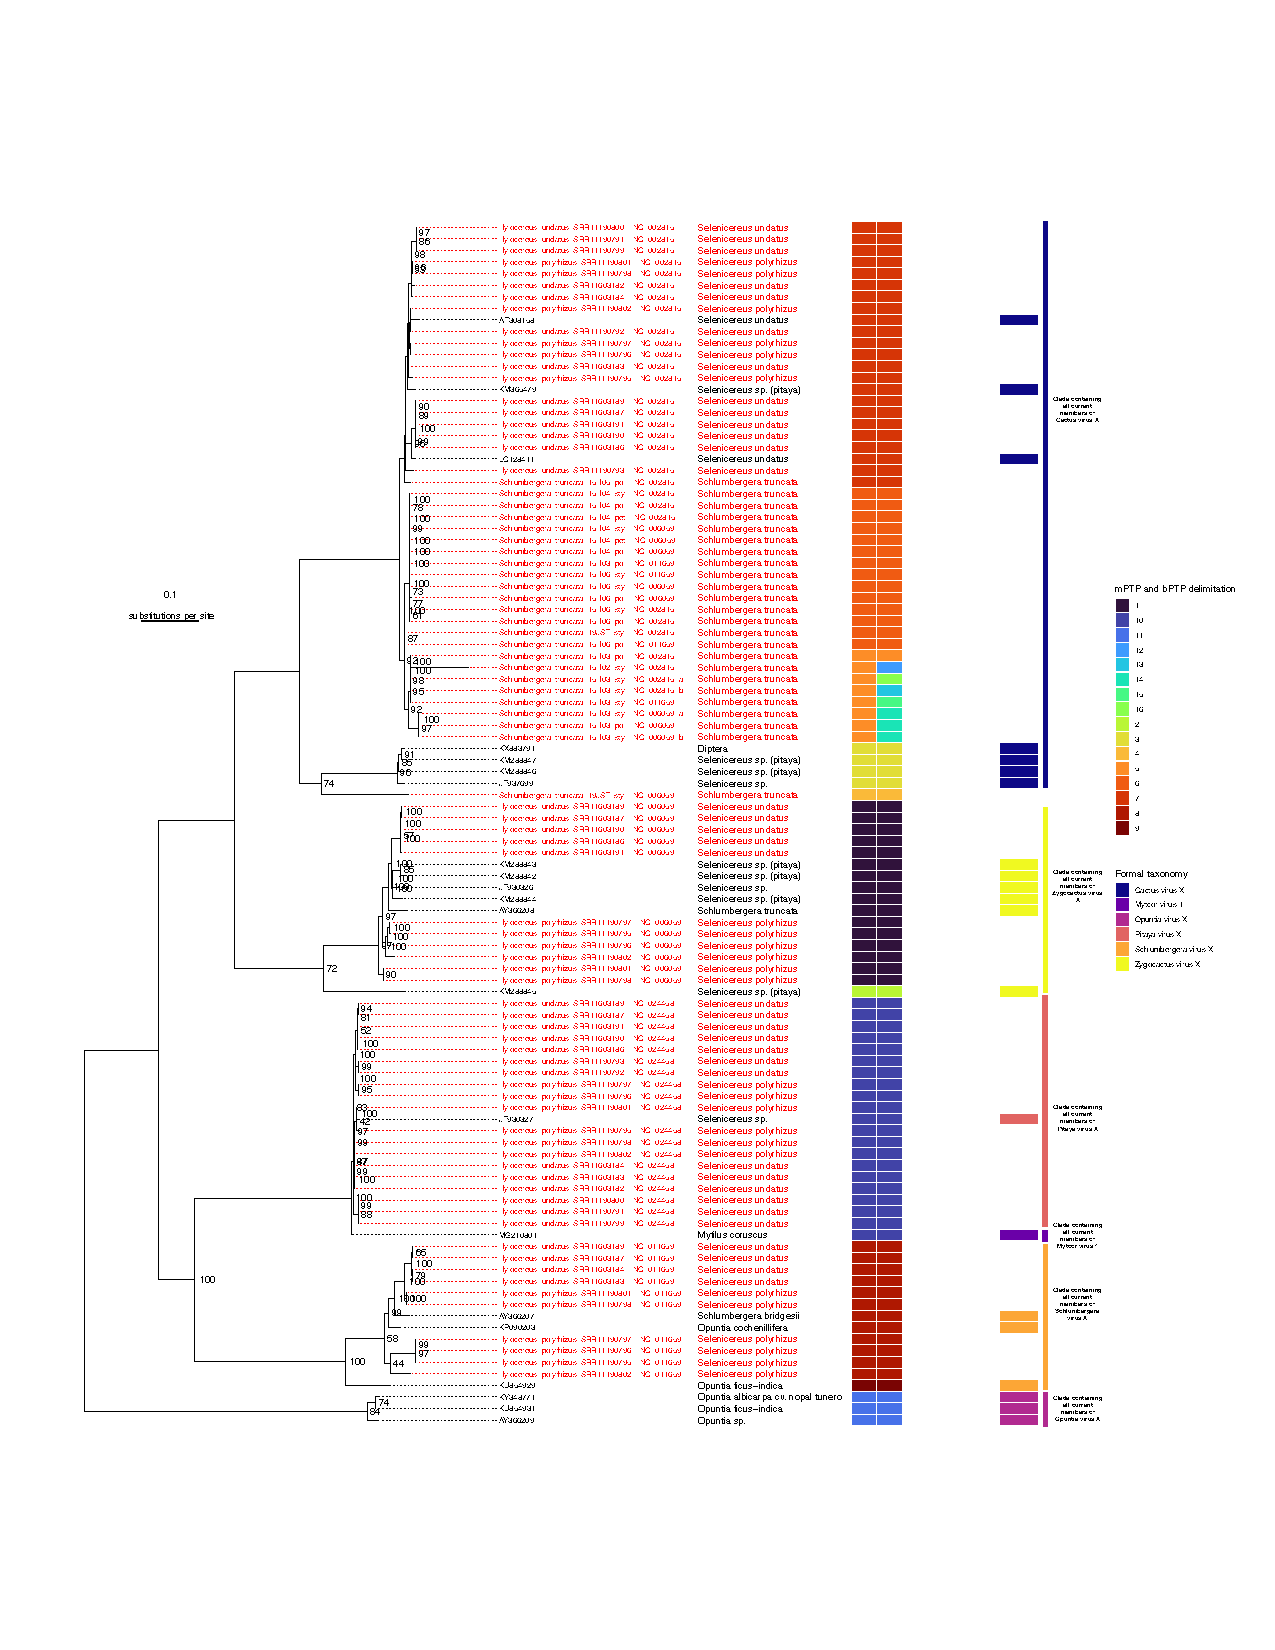
\includegraphics[width=1.0\textwidth]{figures/tree_delim_info.pdf}
\label{fig:tissuetype}
\end{figure}
\clearpage


%%%%%%%%FIGURE 2
\begin{figure}[ht]
\centering
\caption{
Counts of each instance of virus recovered separated by tissue type from within \textit{S. truncata} samples which were assembled during this investigation.
}
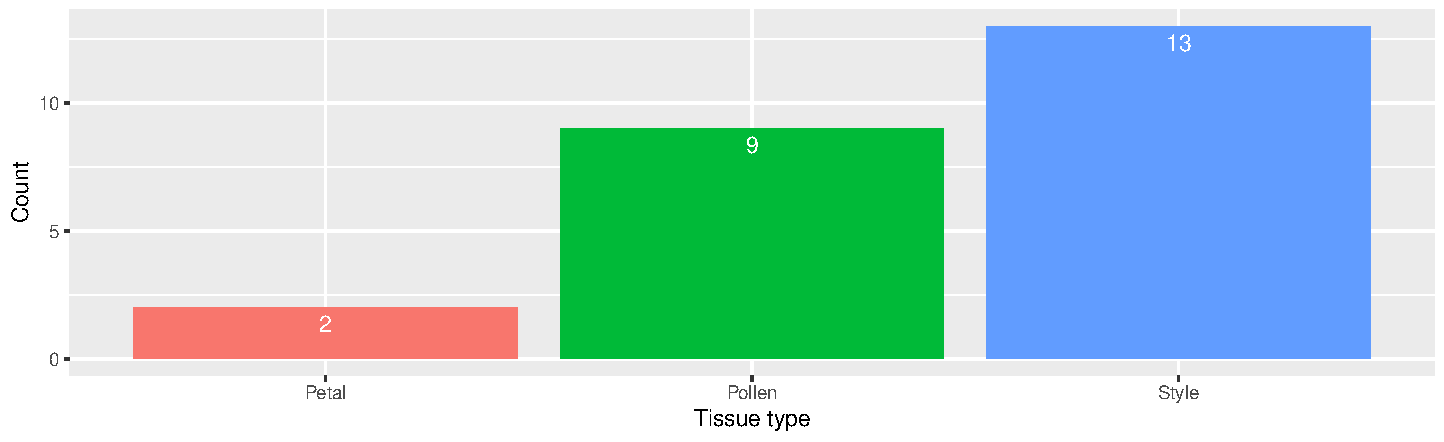
\includegraphics[width=0.7\textwidth]{figures/tistype}
\label{fig:tissuetype}
\end{figure}

%%%%%%%%FIGURE 3
\begin{figure}[ht]
\centering
\caption{
Plot of selection analysis indicating positive selection (dN/dS greater than 1) on areas of the viral genome.
}
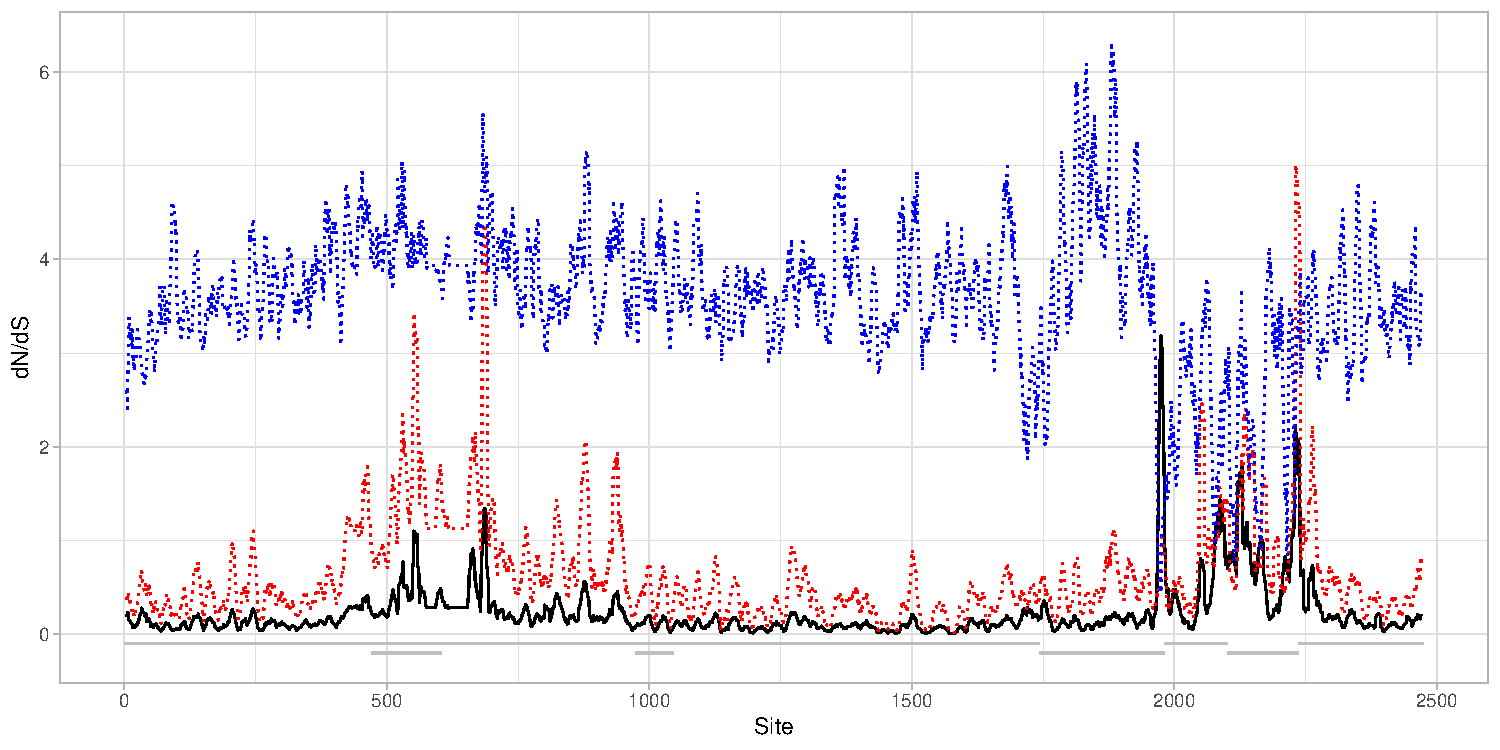
\includegraphics[width=1.0\textwidth]{figures/selectionplot.pdf}
\label{fig:tissuetype}
\end{figure}
\clearpage

%%%%%%%%FIGURE 4
\begin{figure}[ht]
\centering
\caption{
Heatmap of raw sequence distances with pairwise deletion of sites with a missing or gap character. A complete hierarchical clustering tree is displayed above and to the side of the heatmap. Formal taxonomy, when available, is noted on the tips of the clustered tree. 
}
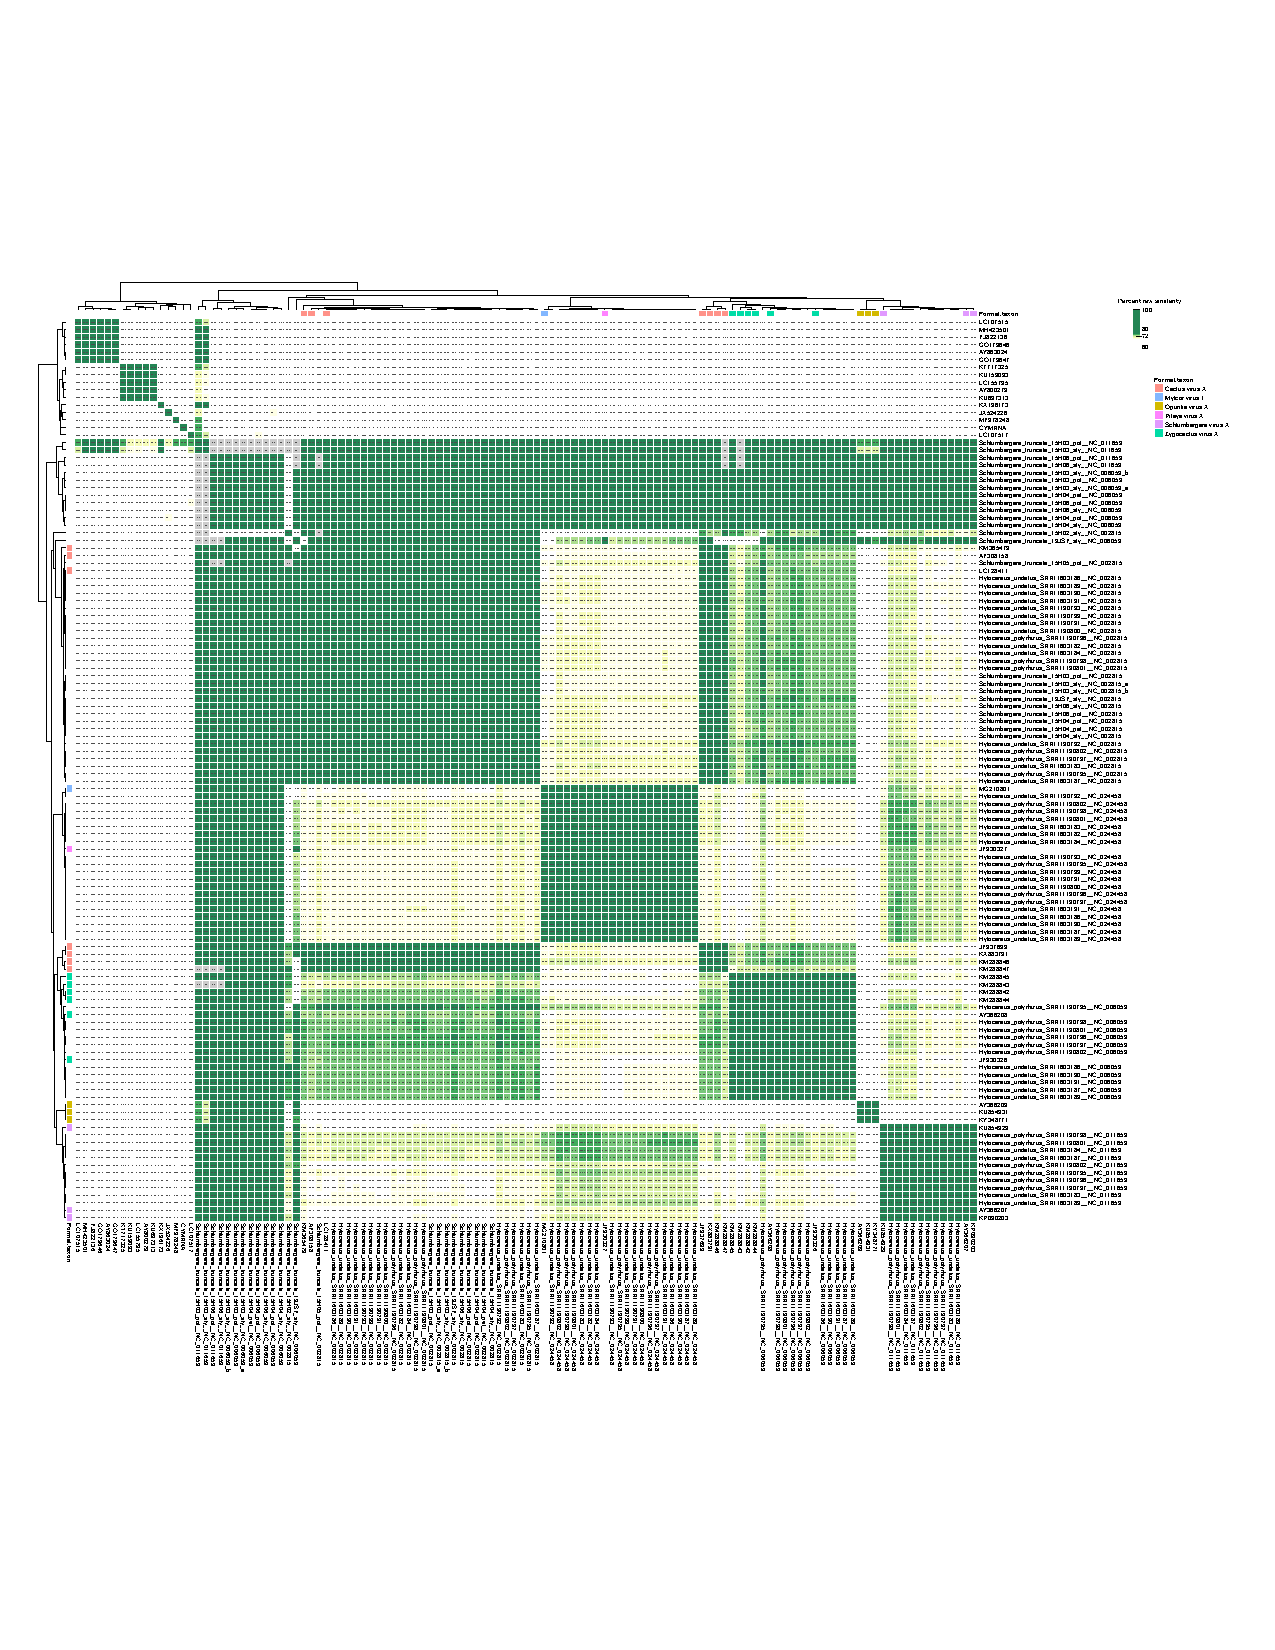
\includegraphics[width=1.0\textwidth]{figures/heatmap-rawseqdist-ed.pdf}
\label{fig:tissuetype}
\end{figure}
\clearpage


% \begin{figure}[ht]
% \centering
% \includegraphics[width=0.5\linewidth]{FILE_PATH}
% \begin{NoHyper}
% \caption{{\fontsize{10pt}{11pt}\selectfont}
% \label{fig:FIG_LABEL}
% \end{NoHyper}
% \end{figure}

% END =========================================================================

\end{document}
